\section{具体实现}

\subsection{CPU模块}

CPU模块无可厚非是我们本次实现中最重要的一个模块,这个模块里面包含了非常多的原件,我们使用了如下组件来实现我们整个CPU。下面会一一列举。

\begin{center}
    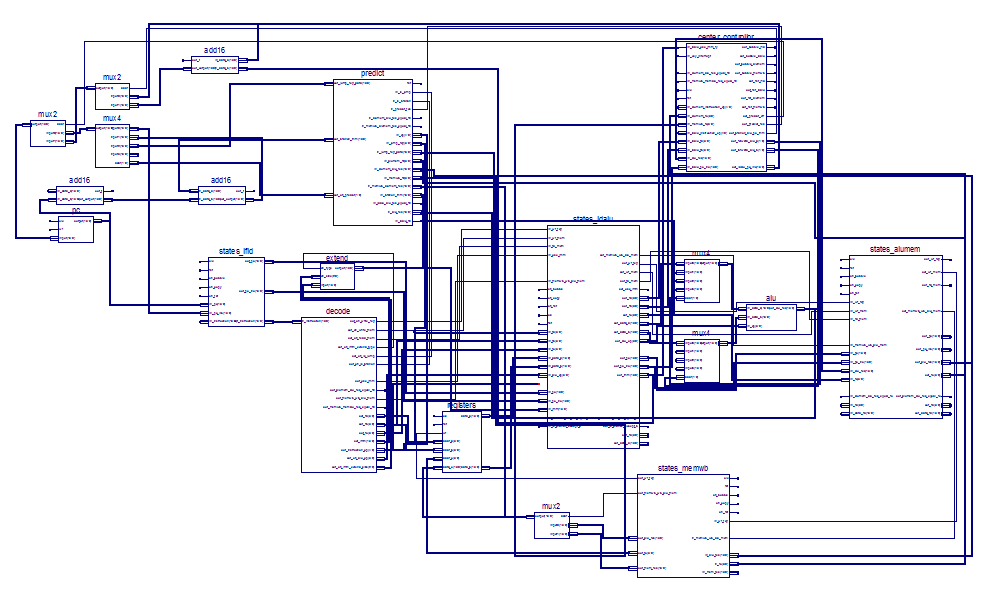
\includegraphics[height=10cm]{image/detail/detail_cpu.png}
    \fcaption{CPU结构图}\label{fig:cpu_structure}
\end{center}

\subsubsection{锁存单元}

锁存单元包含if/id阶段,id/alu阶段,alu/mem阶段,mem/wb阶段四个大的锁存器,在上升沿触发。这几个锁存器的行为都受到中央控制单元的控制,中央控制单元可以命令其进行气泡的插入,以及重置功能。

这四个部件的图如\fref{fig:ifid}-\fref{fig:idalu}所示,具体信号如\tref{table:ifid}-\tref{table:idalu}所示。

\begin{center}
    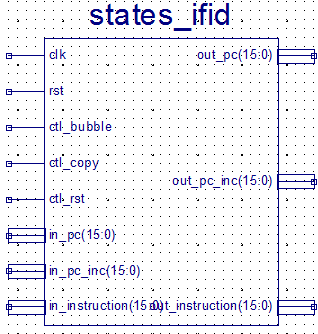
\includegraphics[height=10cm]{image/detail/detail_ifid.png}
    \fcaption{IF/ID阶段锁存器设计图}\label{fig:ifid}
\end{center}

\begin{center}
    \tcaption{IF/ID阶段锁存器信号}\label{table:ifid}
    \begin{longtable}{p{0.2\columnwidth}p{0.8\columnwidth}}
        \toprule
        信号 & 信号描述 \\
        \midrule
        clk & cpu的时钟信号,上升沿的时候根据ctl\_bubble和ctl\_rst进行控制。如果ctl\_bubble和ctl\_rst均为低电平则进行锁存,将in\_pc, in\_pc\_inc, in\_instruction进行锁存并输出。 \\
        rst & 异步清空信号,由外部控制开关接入。 \\
        ctl\_bubble & 气泡控制信号,由中央控制单元给出,如果该信号为高电平则表示下一个时钟上升沿,输出数据保持不变,低电平则该控制无效。 \\
        ctl\_copy &  由中央控制单元给出,用来进行数据拷贝。\\
        ctl\_rst & 重置控制信号,由中央控制单元给出,如果如果该信号为高电平则表示下一个时钟输出清空即为一条NOP指令,低电平则该控制无效。 \\
        in\_pc & 表示下一条将要锁存的指令的pc。 \\
        in\_pc\_inc & 表示下一条将要锁存的指令的pc+1。 \\
        in\_instruction & 表示下一条将要锁存的指令内容 \\
        out\_pc & 表示已经锁存的指令的pc。 \\
        out\_pc\_inc & 表示已经锁存的指令的pc+1。 \\
        out\_instruction & 表示已经锁存的指令。 \\
        \bottomrule
    \end{longtable}
\end{center}

\begin{center}
    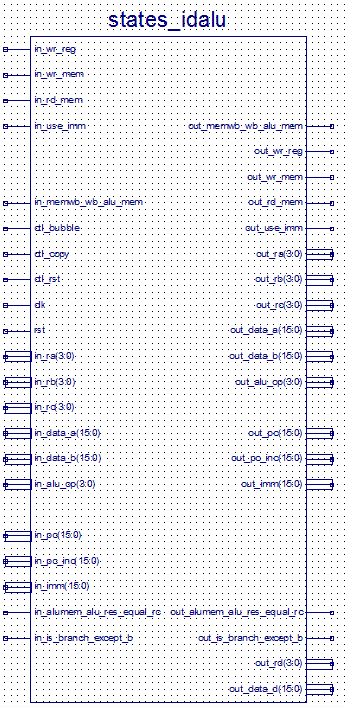
\includegraphics[height=10cm]{image/detail/detail_idalu.png}
    \fcaption{ID/ALU阶段锁存器设计图}\label{fig:idalu}
\end{center}

\begin{center}
    \tcaption{ID/ALU阶段锁存器信号}\label{table:idalu}
    \begin{longtable}{p{0.2\columnwidth}p{0.8\columnwidth}}
        \toprule
        信号 & 信号描述 \\
        \midrule
        in\_ra  & 这是下一条指令decode出来的alu操作数a的寄存器值,注意不是数值,会传递给中央控制单元进行旁路选择。 \\
        % 用来传输给选择器最后送到alu进行计算
        in\_rb &  这是下一条指令decode出来的alu操作数b的寄存器值,注意不是数值,会传递给中央控制单元进行旁路选择。\\
        in\_rc &  这是下一条指令decode出来的寄存器c的值,注意不是数值,会传递给中央控制单元进行旁路选择,也会传递给alumem锁存器。c的寄存器表示的
        是写回的寄存器,非常重要,所以要一直往后传。\\
        in\_data\_a &  这是下一条指令decode出来的alu操作数a的值,用来传输给选择器,(选择器可能会选择旁路),最后送到alu进行计算。 \\
        in\_data\_b &  这是下一条指令decode出来的alu操作数b的值,用来传输给选择器,(选择器可能会选择旁路),最后送到alu进行计算。 \\\\
        in\_alu\_op &  这是下一条指令alu的操作码,会传输给三个alu,具体内容请看alu部分。\\
        in\_pc &  表示下一条将要锁存的指令的pc。\\
        in\_pc\_inc &  表示下一条将要锁存的指令的pc+1。\\
        in\_imm &  表示下一条将要锁存的decode出来的立即数。\\
        in\_wr\_reg &  表示下一条指令是否需要在writeback阶段写回寄存器。\\
        in\_wr\_mem &  表示下一条指令是否需要在memory阶段写内存。\\
        in\_rd\_mem &  表示下一条指令是否需要在memory阶段读内存。\\
        in\_use\_imm & 表示下一条指令在alu阶段是否需要使用立即数,这个信号会帮助中央控制单元进行alu\_data\_b旁路的控制。 \\
        in\_alumem\_alu\_  res\_equal\_rc &  表示下一条指令到memory阶段的时候,alu的出的结果是否会在writeback阶段写回寄存器。这个信号也是为了帮助中央控制单元进行旁路控制。\\
        in\_memwb\_wb\_  alu\_mem &  表示下一条指令在writeback阶段写回的数据是memory阶段读出的数据,还是在alu阶段算出的结果。\\
        in\_is\_branch\_  except\_b & 表示下一条指令是否是branch指令,除了b指令以外的branch指令都是高电平,这个信号是帮助中央控制单元进行分支预测的检验使用的信号。 \\
        ctl\_bubble &  气泡控制信号,由中央控制单元给出,如果该信号为高电平则表示下一个时钟上升沿,输出数据保持不变,低电平则该控制无效。\\
        ctl\_copy &  由中央控制单元给出,用来进行数据拷贝。\\
        ctl\_rst &  重置控制信号,由中央控制单元给出,如果如果该信号为高电平则表示下一个时钟输出清空即为一条NOP指令,低电平则该控制无效。\\
        clk &  cpu的时钟信号,上升沿的时候根据ctl\_bubble和ctl\_rst进行控制。如果ctl\_bubble和ctl\_rst均为低电平则进行锁存,将所有带有out前轴的信号对应的in信号锁存然后输出。\\
        rst &  异步清空信号,由外部控制开关接入。\\
        out\_ra &  表示alu阶段运算的寄存器a的值,这个值会送到中央控制单元进行旁路的控制。\\
        out\_rb &  表示alu阶段运算的寄存器b的值,这个值会送到中央控制单元进行旁路的控制。\\
        out\_rc &  表示writeback阶段写回的寄存器c的值。\\
        out\_rd &  rd是一个特殊的输出,只会在sw这条指令进行使用,rd也需要送到中央控制单元进行旁路的控制,他的内容和rb完全一致。\\
        out\_data\_a &  表示alu阶段运算a的值,这个值是从一个四选一的选择器得到的,这个选择器的控制由中央控制单元给出。\\
        out\_data\_b &  表示alu阶段运算b的值,这个值是从一个四选一的选择器得到的,这个选择器的控制由中央控制单元给出。\\
        out\_data\_d &  表示memory阶段sw指令可能用到的值,这个值是从一个四选一的选择器得到的,这个选择器的控制由中央控制单元给出。\\
        out\_alu\_op &  表示当前alu进行的运算符号。\\
        out\_pc &  表示已经锁存的指令的pc。\\
        out\_pc\_inc &  表示已经锁存的指令的pc+1。\\
        out\_imm &  表示已经锁存的指令的立即数,这个数字会连接到alu\_data\_b的选择器。\\
        out\_alumem\_alu\_  res\_equal\_rc &  表示当前指令到memory阶段的时候,alu的出的结果是否会在writeback阶段写回寄存器。这个信号也是为了帮助中央控制单元进行旁路控制。\\
        out\_memwb\_wb\_  alu\_mem &  表示当前指令在writeback阶段写回的数据是memory阶段读出的数据,还是在alu阶段算出的结果。\\
        out\_is\_branch\_  except\_b &  表示当前指令是否是branch指令,除了b指令以外的branch指令都是高电平,这个信号是帮助中央控制单元进行分支预测的检验使用的信号。\\
        out\_wr\_reg &  表示当前指令是否需要在writeback阶段写回寄存器。\\
        out\_wr\_mem &  表示当前指令是否需要在memory阶段写内存。\\
        out\_rd\_mem &  表示当前指令是否需要在memory阶段读内存。\\
        out\_use\_imm & 表示当前指令在alu阶段是否需要使用立即数,这个信号会帮助中央控制单元进行alu\_data\_b旁路的控制。 \\
        \bottomrule
    \end{longtable}
\end{center}

\begin{center}
    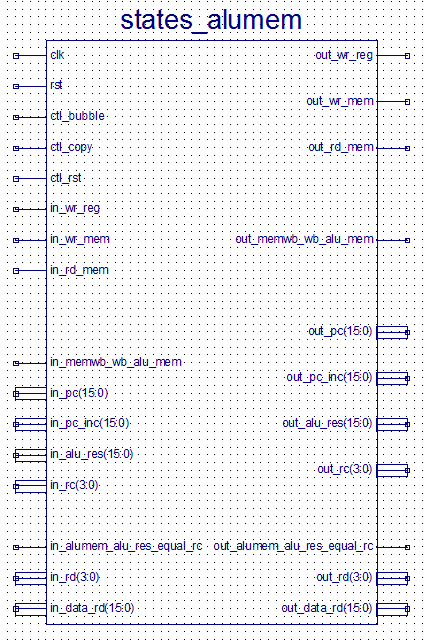
\includegraphics[height=10cm]{image/detail/detail_alumem.png}
    \fcaption{ALU/MEM阶段锁存器设计图}\label{fig:alumem}
\end{center}

\begin{center}
    \tcaption{ALU/MEM阶段锁存器信号}\label{table:alumem}
    \begin{longtable}{p{0.2\columnwidth}p{0.8\columnwidth}}
        \toprule
        信号 & 信号描述 \\
        \midrule
        in\_rc &  这是下一条指令decode出来的寄存器c的值,注意不是数值,会传递给中央控制单元进行旁路选择,也会传递给memwb锁存器。c的寄存器表示的
        是写回的寄存器,非常重要,所以要一直往后传。\\
        in\_rd & 这是专门为了sw指令设计的寄存器的值。\\ 
        in\_data\_rd & 这是专门为了sw指令设计的寄存器的值,通过一个4️选1选择可以确保数据的正确性。由于我们的设计问题,alu在进行sw指令的时候无法将sw的源寄存器值进行旁路计算解决数据冲突,所以使用了单独的一条旁路来解决这个问题。\\
        in\_pc &  表示下一条将要锁存的指令的pc。\\
        in\_pc\_inc &  表示下一条将要锁存的指令的pc+1。\\
        in\_wr\_reg &  表示下一条指令是否需要在writeback阶段写回寄存器。\\
        in\_wr\_mem &  表示下一条指令是否需要在memory阶段写内存。\\
        in\_rd\_mem &  表示下一条指令是否需要在memory阶段读内存。\\
        in\_alu\_res & 表示下一条指令alu得出的结果。\\
        
        
        in\_alumem\_alu\_  res\_equal\_rc & 表示下一条指令alu计算出的结果是否会在writeback阶段写回寄存器。这个信号也是为了帮助中央控制单元进行旁路控制。\\
        in\_memwb\_wb\_  alu\_mem & 表示下一条指令在writeback阶段写回的数据是memory阶段读出的数据,还是在alu阶段算出的结果。\\
        clk & cpu的时钟信号,上升沿的时候根据ctl\_bubble和ctl\_rst进行控制。如果ctl\_bubble和ctl\_rst均为低电平则进行锁存,将所有带有out前轴的信号对应的in信号锁存然后输出。\\
        rst & 异步清空信号,由外部控制开关接入。\\
        ctl\_bubble &  气泡控制信号,由中央控制单元给出,如果该信号为高电平则表示下一个时钟上升沿,输出数据保持不变,低电平则该控制无效。\\
        ctl\_copy &  由中央控制单元给出,用来进行数据拷贝。\\
        ctl\_rst &  重置控制信号,由中央控制单元给出,如果如果该信号为高电平则表示下一个时钟输出清空即为一条NOP指令,低电平则该控制无效。\\
        out\_pc &  表示已经锁存的指令的pc。\\
        out\_pc\_inc &  表示已经锁存的指令的pc+1。\\
        out\_alu\_res & 表示当前指令在alu阶段通过alu计算出来的值。\\
        out\_rc & 表示当前指令decode出来的目的寄存器c的值。\\
        out\_wr\_reg &  表示当前指令是否需要在writeback阶段写回寄存器。\\
        out\_wr\_mem &  表示当前指令是否需要在memory阶段写内存。\\
        out\_rd\_mem &  表示当前指令是否需要在memory阶段读内存。\\
        out\_memwb\_wb\_  alu\_mem & 表示当前指令在writeback阶段写回的数据是memory阶段读出的数据,还是在alu阶段算出的结果。\\
        \bottomrule
    \end{longtable}
\end{center}

\begin{center}
    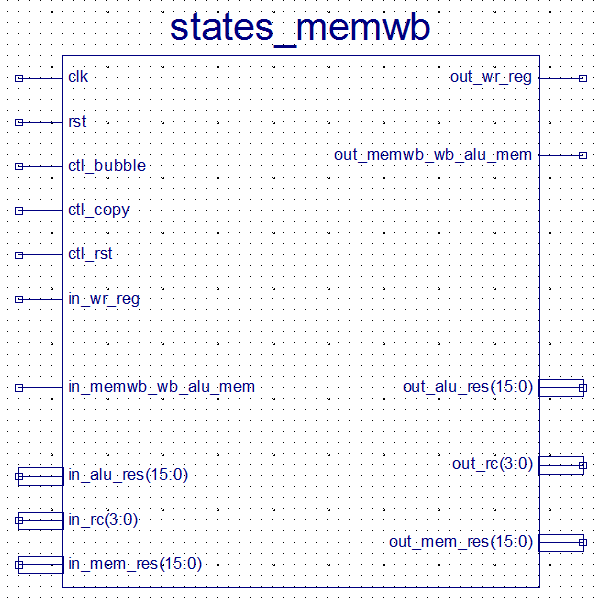
\includegraphics[height=10cm]{image/detail/detail_memwb.png}
    \fcaption{MEM/WB阶段锁存器设计图}\label{fig:memwb}
\end{center}

\begin{center}
    \tcaption{MEM/WB阶段锁存器信号}\label{table:memwb}
    \begin{longtable}{p{0.2\columnwidth}p{0.8\columnwidth}}
        \toprule
        信号 & 信号描述 \\
        \midrule
        clk & cpu的时钟信号,上升沿的时候根据ctl\_bubble和ctl\_rst进行控制。如果ctl\_bubble和ctl\_rst均为低电平则进行锁存,将所有带有out前轴的信号对应的in信号锁存然后输出。\\
        rst & 异步清空信号,由外部控制开关接入。\\
        ctl\_bubble &  气泡控制信号,由中央控制单元给出,如果该信号为高电平则表示下一个时钟上升沿,输出数据保持不变,低电平则该控制无效。\\
        ctl\_copy &  由中央控制单元给出,用来进行数据拷贝。\\
        ctl\_rst &  重置控制信号,由中央控制单元给出,如果如果该信号为高电平则表示下一个时钟输出清空即为一条NOP指令,低电平则该控制无效。\\
        in\_alu\_res & 表示下一条指令alu阶段计算出来的结果,可能用于写回。\\
        in\_rc & 表示下一条指令写回的寄存器值。\\
        in\_wr\_reg & 表示下一条指令是否写回寄存器。\\
        in\_mem\_res & 表示下一条指令memory阶段得到的结果。\\
        in\_memwb\_wb\_ alu\_mem & 表示下一条指令写回寄存器堆的是alu计算的结果还是memory访存的结果。\\
        out\_wr\_reg & 当前指令用来控制寄存器堆的写使能信号,使其可以在下降沿的时候更新。\\
        out\_memwb\_wb\_ alu\_mem & 当前指令写回内容2选1的控制信号,是选择alu计算的结果还是memory访存的结果。\\
        \bottomrule
    \end{longtable}
\end{center}

\subsubsection{PC锁存单元}
    PC锁存器,用来锁存PC,保证PC的改写受到中央控制部分的控制。我们规定在下降沿写入,组合逻辑输出。
    具体信号请看下表。

\begin{center}
    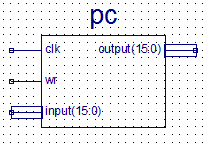
\includegraphics[height=10cm]{image/detail/detail_pc.png}
    \fcaption{PC锁存器}\label{fig:pc}
\end{center}
\begin{center}
    \tcaption{PC锁存器}\label{table:pc}
    \begin{longtable}{p{0.2\columnwidth}p{0.8\columnwidth}}
        \toprule
        信号 & 信号描述 \\
        \midrule
            input & 表示修改信号的输入,即修改的值。\\
            clk & CPU时钟。\\
            wr & 修改使能,如果为高电平则在下降沿修改pc的锁存器的值。\\
            rst & 异步清空信号,由外部控制开关接入。\\
            output & 当前pc锁存的值,组合逻辑。\\
        \bottomrule
    \end{longtable}
\end{center}

下一条PC的选择是一个非常复杂的结构,具体的原理图如下。
\begin{center}
    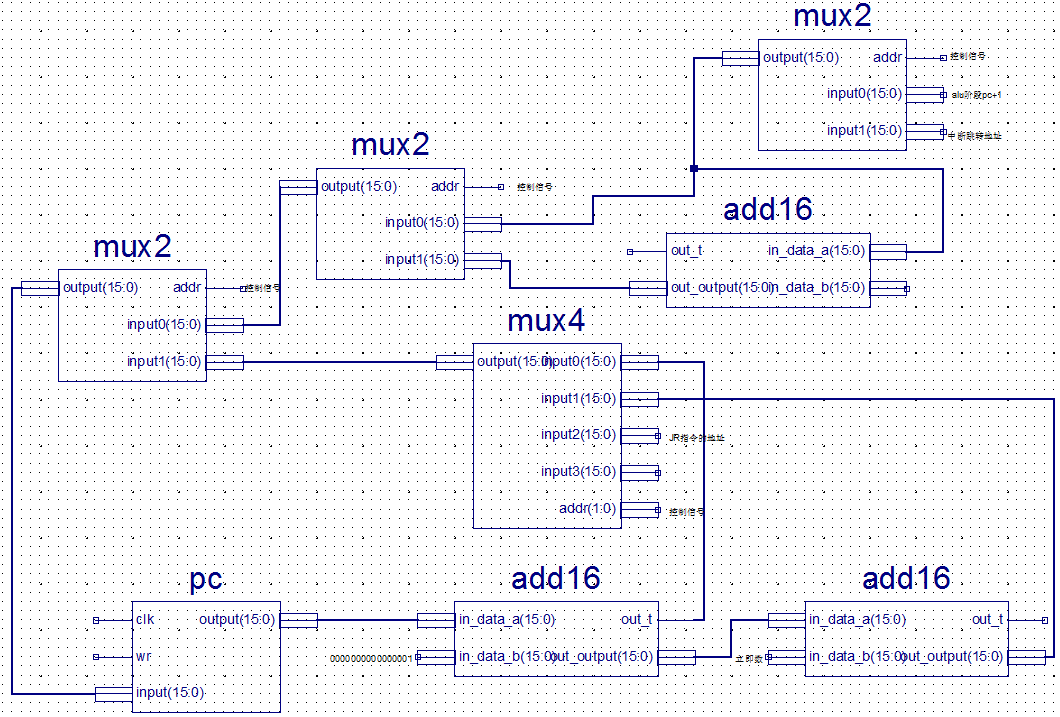
\includegraphics[height=10cm]{image/detail/detail_pc_structure.png}
    \fcaption{PC结构图}\label{fig:pcstructure}
\end{center}
具体而言,PC的选择由两条路线决定。
\begin{enumerate}
    \item 在decode阶段进行的跳转,包含jr指令以及分支预测。这里使用了图中下部分的部件,4选1的选择器可以选择pc+1,pc+1+imm,reg的值进行跳转。控制信号都是中央控制单元给出的。
    \item 在alu发现分支预测错误或者进行中断的跳转,则在上部分,最右边是一个2选1,选择进行跳转的基础地址是alu阶段的记录下来的pc地址,或者是中断的指令的地址,左边的2选1则是是否加上立即数的选择器,最后连向最左边的2选1选择器。
\end{enumerate}
综合上面的结构,构成了我们的pc整个模块,是的cpu的跳转可以正常的工作。
由于大部分控制信号都是有中央控制单元给出,控制信号将统一在中央控制器里面描述。

\subsubsection{跳转单元}
    跳转单元,用来在decode阶段进行计算和控制跳转的目的地址,这里面有旁路来处理JR指令的数据冲突。
    具体信号请看下表。
\begin{center}
    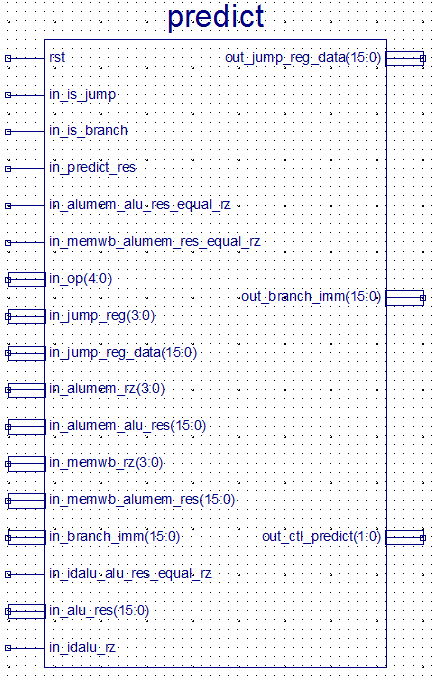
\includegraphics[height=10cm]{image/detail/detail_predict.png}
    \fcaption{跳转单元}\label{fig:predict}
\end{center}
\begin{center}
    \tcaption{跳转单元}\label{table:predict}
    \begin{longtable}{p{0.2\columnwidth}p{0.8\columnwidth}}
        \toprule
        信号 & 信号描述 \\
        \midrule
            rst & 异步清空信号,由外部控制开关接入。\\
            in\_is\_jump & 由decode给出的当前指令是不是jump指令。\\
            in\_is\_b & 由decode给出的当前指令是不是b指令。\\
            in\_is\_branch\_  except\_b & 由decode给出的当前指令是不是除了b的branch指令。 \\
            in\_predict\_res & 由中央控制单元给出的分支预测的结果。\\
            in\_jump\_reg & 由decode给出的jr指令的寄存器的值。\\
            in\_jump\_reg\_  data & 由寄存器堆给出的jr指令的寄存器的数据。\\
            in\_idalu\_alu\_  res\_equal\_rc & 这是为旁路设计的,用来计算alu阶段出现的数据冲突,这个信号表示alu阶段alu的值会在最后写回c寄存器。\\
            in\_idalu\_rc & 当前alu阶段c寄存器的值。\\
            in\_alu\_res & 当前alu阶段alu的值。\\
            in\_alumem\_rc & 当前alu阶段c寄存器的值。\\
            in\_alumem\_alu\_  res\_equal\_rc & 这是为旁路设计的,用来计算mem阶段出现的数据冲突,这个信号表示mem阶段alu的值会在最后写回c寄存器。\\
            in\_alumem\_alu\_  res & 当前memory阶段alu的值。\\
            in\_memwb\_rc & 当前writeback写回的寄存器c的值。\\
            in\_memwb\_alumem  \_res\_equal\_rc & 这是为旁路设计的,用来计算mem阶段出现的数据冲突,这个信号表示writeback阶段alu或者mem的值会在最后写回c寄存器。\\
            in\_memwb\_alumem  \_res & writeback阶段写回的值。\\
            in\_branch\_imm & 这个数据表示branch指令立即数的值,将会给pc模块用来进行加法。\\
            out\_jump\_reg\_  data & 这个输出用来连接到pc模块里面的4选1选择器,表示jr指令的目的地值。\\
            out\_branch\_imm & 这个数据用来输出表示branch指令立即数的值,将会给pc模块用来进行加法。\\
            out\_ctl\_predict & 这个数据用来输出表示分支预测的结果,连接到选择器上。\\
        \bottomrule
    \end{longtable}
\end{center}
    

\subsubsection{寄存器堆}
    寄存器堆用来输出寄存器的值,以及在时钟下降沿提供修改寄存器值的功能。
    具体信号请看下表。
\begin{center}
    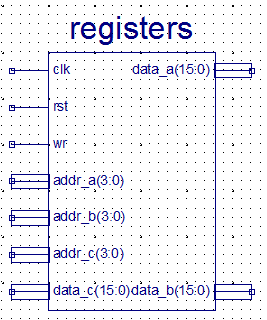
\includegraphics[height=10cm]{image/detail/detail_register.png}
    \fcaption{寄存器堆}\label{fig:register}
\end{center}
\begin{center}
    \tcaption{寄存器堆}\label{table:register}
    \begin{longtable}{p{0.2\columnwidth}p{0.8\columnwidth}}
        \toprule
        信号 & 信号描述 \\
        \midrule
            clk & CPU时钟信号。\\
            rst &  异步清空信号,由外部控制开关接入。\\
            wr & 寄存器堆写使能,如果为高电平则在clk下降沿的时候将data\_c写入对应的addr\_c里面。\\
            addr\_a & 接受decode出来的寄存器a。\\
            addr\_b & 接受decode出来的寄存器b。\\
            addr\_c & 接受writeback将要写回的寄存器c。\\
            data\_a & 输出decode出来的寄存器a的数值。\\
            data\_b & 输出decode出来的寄存器b的数值。\\
            data\_c & 写回阶段修改寄存器的值。\\
        \bottomrule
    \end{longtable}
\end{center}

